\chapter{Artefact Design}

\section{Introduction} \label{a-d--introduction}

In Chapter 2 we identified that blah blah...
This chapter describes the design of blah blah, a system that blah blah.  First, the chapter describes the project’s design methodology (section 3.2), and system requirements (section 3.3).  A proposed solution is then discussed (section 3.4), followed by a blah blah....


\section{Design Methodology} \label{a-d--methodology}

The design and development of blah blah

\subsection{A Review of Existing Software} \label{a--d--review-of-existing-software}

This section is a review of current homebrewing software.

\subsubsection{BeerSmith}

+ Cross platform (Macintosh, Ubuntu and Windows)

\subsubsection{BeerTools Pro}
\subsubsection{Beer Calculus}
\subsubsection{ProMash}
\subsubsection{BrewPal}
\subsubsection{BrewTarget}
\subsubsection{BeerAlchemy}
\subsubsection{Brewer's Friend}

% Need to review the rest of the brewing software https://homebrew.stackexchange.com/questions/784/what-software-do-most-brewers-use/898]

One thing that is common among all of these choices is their inherent offline nature. As they are installed directly to the computer and not in a web browser.

\subsection{Software Life-cycle Methodology} \label{a-d--methodology--life-cycle}

Choosing a methodology is never one size fits all. Instead considering the environment and team around a project is important. Agile software development offers principles that work well with a team, however there is a lot that can be taken for any project.

Agile development embraces changes in development life-cycle and adapts to them, this is in contrast to tradtional plan-driven development in which predictions are used instead. An agile plan is the initial set of goals which will adapt as the project grows. \cite{fowler_agile}

Using an incremental and evolutionary approach is key for this artefact due to it's experimental nature, the goals and proposed solutions will change through-out development.

\subsection{Tools and Services} \label{a-d--methodology--tools}

Kanban boards are a tool to visualise the workflow for a project, an online implementation of this tool is Trello. Trello can be used for multiple scenarios and fits well for a software project. Features, bugs and other research can be represented by cards. \cite{trello} % cite for kanban

Version control is arguably one of the most important tools in software development. It records changes over time so that a previous version of the project can be revisited later. Git is a free and open source distributed version control system that is used on many projects. \cite{git}

While being distributed it's often useful to have a centralized repository, there are many Git repository hosting services. GitHub and Bitbucket are two popular choices. While GitHub encourages Open Source Software on their platform the service itself isn't Open Source. \cite{github} GitLab started as a GitHub clone that is fully Open Source, with the choice to host yourself or use their servers. \cite{gitlab} \cite{bitbucket}

These platforms offer similar features but the artefact will be hosted with GitHub due to the familiarity to the author and also the features it offers.

GitHub has a system of `Issues', which allow for tasks to be tracked. These issues can be commented and then closed when deemed completed. For this project the following labels are used:

\begin{itemize}
  \item \textbf{\colorbox{red}{bug}} - tasks which define a bug in the project
  \item \textbf{\colorbox{blue}{feature}} -  tasks which introduce a new feature to the project
  \item \textbf{\colorbox{yellow}{report}} - tasks which are relevant to the report writing itself
  \item \textbf{\colorbox{green}{greenkeeper}} - a label reserved for the greenkeeper tool (as described in x of this report)
  \item \textbf{wontfix} - tasks that are out of scope and/or outdated and wont be completed
\end{itemize}

Following is a screenshot of the issues at one point in the project:

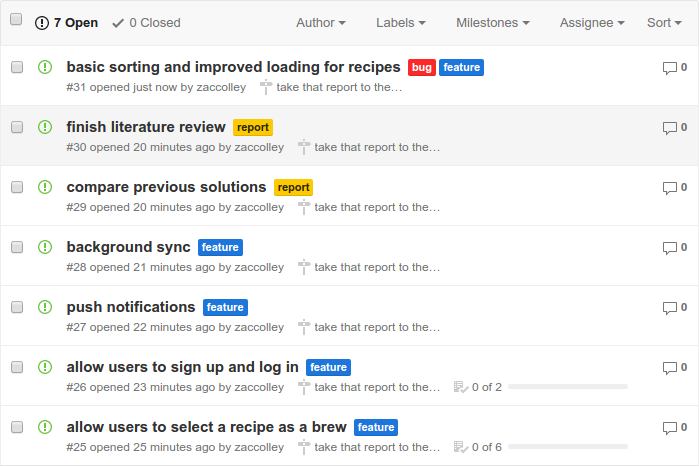
\includegraphics[width=\textwidth,height=\textheight,keepaspectratio]{githubissues}
% have this as a figure?

\section{Requirements} \label{a-d--requirements}

Both the supervisor Rich Boakes and local Portsmouth homebrewer Alan Thompson of GetBrewing.uk, fueled the initial requirements for this project. They saw a need for applications that help improve the current homebrewing ecosystem.

As follows are requirements to create such a application to improve the brewing process when following recipes. After reviewing the current software available in section \ref{a--d--review-of-existing-software} it is clear there are problems in these areas:

\begin{itemize}
  \item Blah
  \item Blah
  \item Blah
  \item Blah
\end{itemize}

One key aspect from a lot of this software is as it is installed to a computer it is offline. Something a tradtional web app couldn't achieve. Having the artefact introduce offline features makes for an innovative solution.

This application will look to solve some of these issues.

\subsection{Functional Requirements} \label{a-d--requirements--functional}

The following requirements will be structured through user stories. % cite

\subsubsection{Finding recipes}

\begin{itemize}
  \item As a \textbf{user}, I want to \textbf{search for recipes by recipe and name and description}
  \item As a \textbf{user}, I want to \textbf{browse for recipes by different recipe categories}
\end{itemize}

\subsubsection{Starting a brew}

\begin{itemize}
  \item As a \textbf{user}, I want to \textbf{select and start a brew from any recipe}
\end{itemize}

\subsubsection{Managing a brew}

\begin{itemize}
  \item As a \textbf{user}, I want to \textbf{manage the ingredients for a brew}
  \item As a \textbf{user}, I want to \textbf{be reminded at key stages of a brew}
  \item As a \textbf{user}, I want to \textbf{add notes to key stages of a brew}
  \item As a \textbf{user}, I want to \textbf{review and evaluate the brew on completion}
\end{itemize}

\subsection{Non-Functional Requirements} \label{a-d--requirements--non-functional}

The artefact should:

\begin{itemize}
  \item Follow accessiblity guidelines to ensure usage for those of hard of sight
  \item Be documented so that others can maintain
  \item Conform to the performance budget that is set in inital development
  \item Work in specified browser, operating system and screen size environment: x
  \item Pass tests generated throughout and running through continuous integration (such as Travis CI)
\end{itemize}

\section{Proposed Solution} \label{a-d--proposed-solution}

Blah blah blah at a high level, then create subsections that go into detail

% using node

% using a virtual dom

% no web fonts, images, svg over font icons. interesting style and type usage wins over

\section{Summary} \label{a-d--summary}

This chapter described the high-level requirements and design of a system that blah blah blah.  The chapter started by describing blah.  The proposed solution was then discussed in section blah followed by blah in section blah, etc.
Blah blah is covered in further detail in Chapter 4 which describes the implementation of blah blah.
